%
% ---- System Architectures
%

\section{System architectures}

The proposed system will use distributed architectures.  Users will access it from a web-based front end.  Tickets will be stored in a database partitioned across several data nodes.  In between the web servers and database will be a number of worker applications to service user requests, connected to the web servers by some middleware.

\begin{figure}
	\caption{Ticketing application distributed architecture 1}
	\centering
	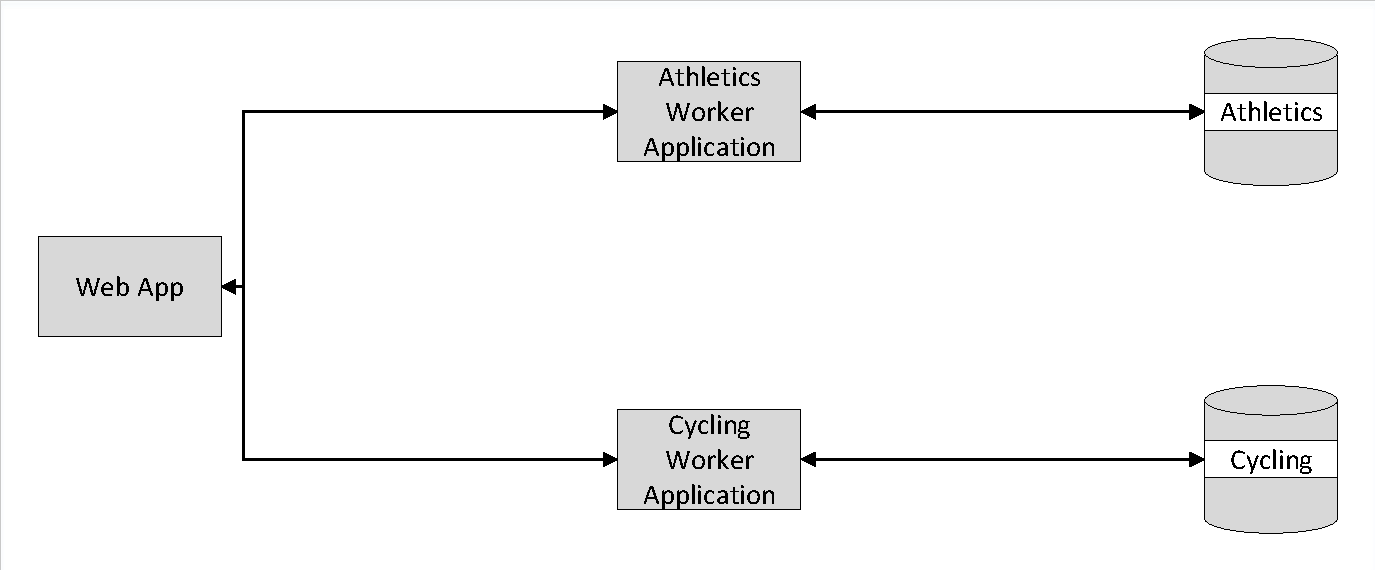
\includegraphics[trim = 5 5 5 5, clip, width=\textwidth]{img/simplemicro}
\end{figure}

\begin{figure}
	\caption{Ticketing application distributed architecture 2}
	\centering
	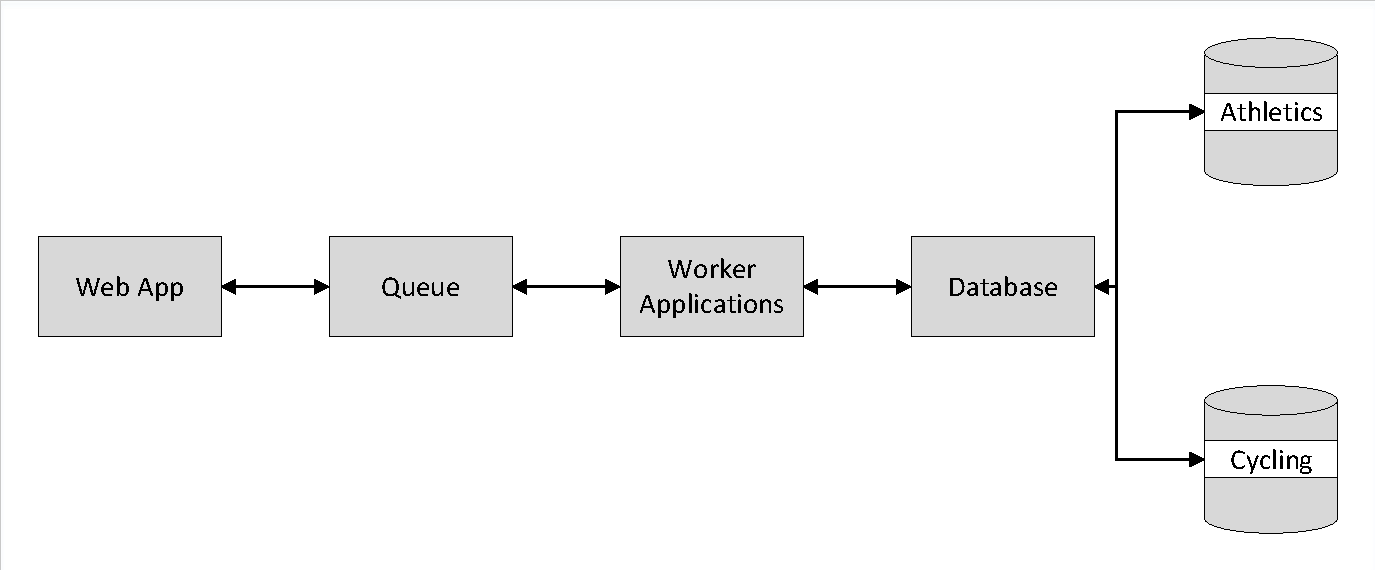
\includegraphics[trim = 5 5 5 5, clip, width=\textwidth]{img/sharedqueue}
\end{figure}

\begin{figure}
	\caption{Ticketing application distributed architecture 3}
	\centering
	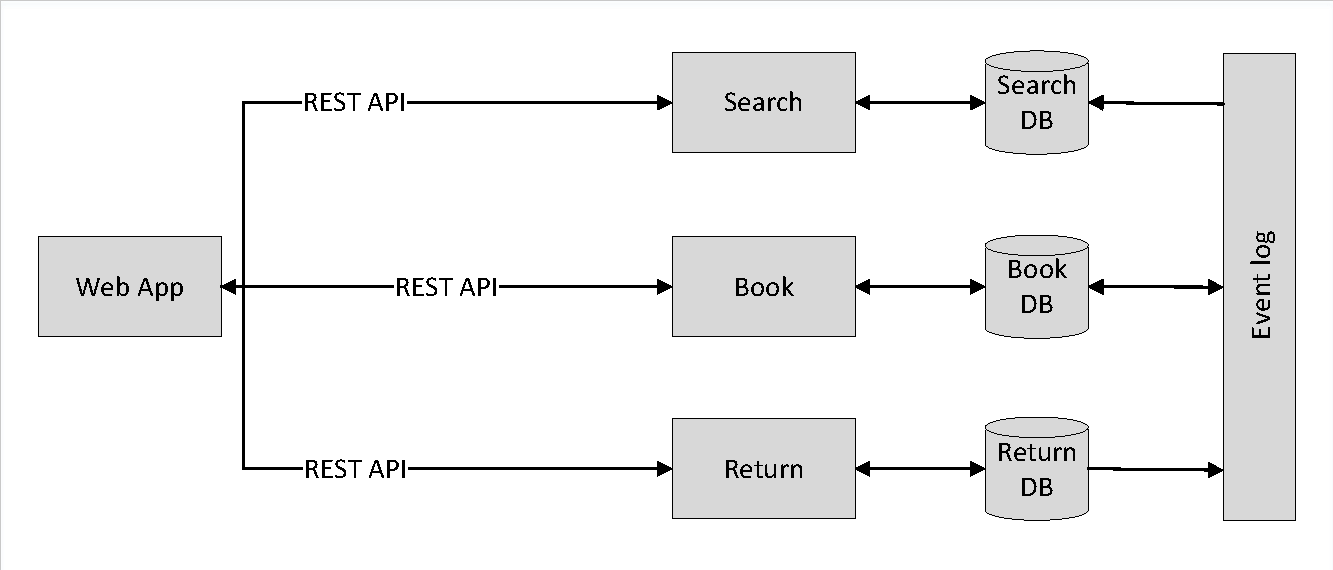
\includegraphics[trim = 5 5 5 5, clip, width=\textwidth]{img/operationmicro}
\end{figure}

\begin{figure}
	\caption{Ticketing application distributed architecture 4}
	\centering
	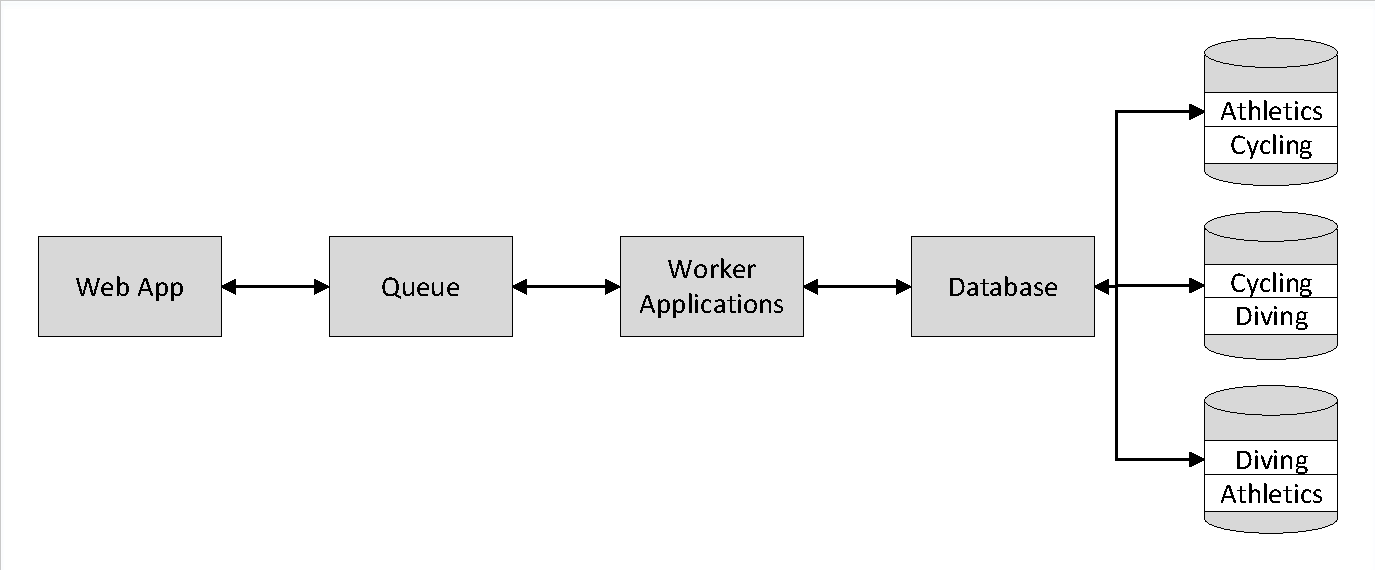
\includegraphics[trim = 5 5 5 5, clip, width=\textwidth]{img/sharedqueue_withrep}
\end{figure}